\documentclass{standalone}
\usepackage{tikz}
\usetikzlibrary{patterns, positioning}

\begin{document}
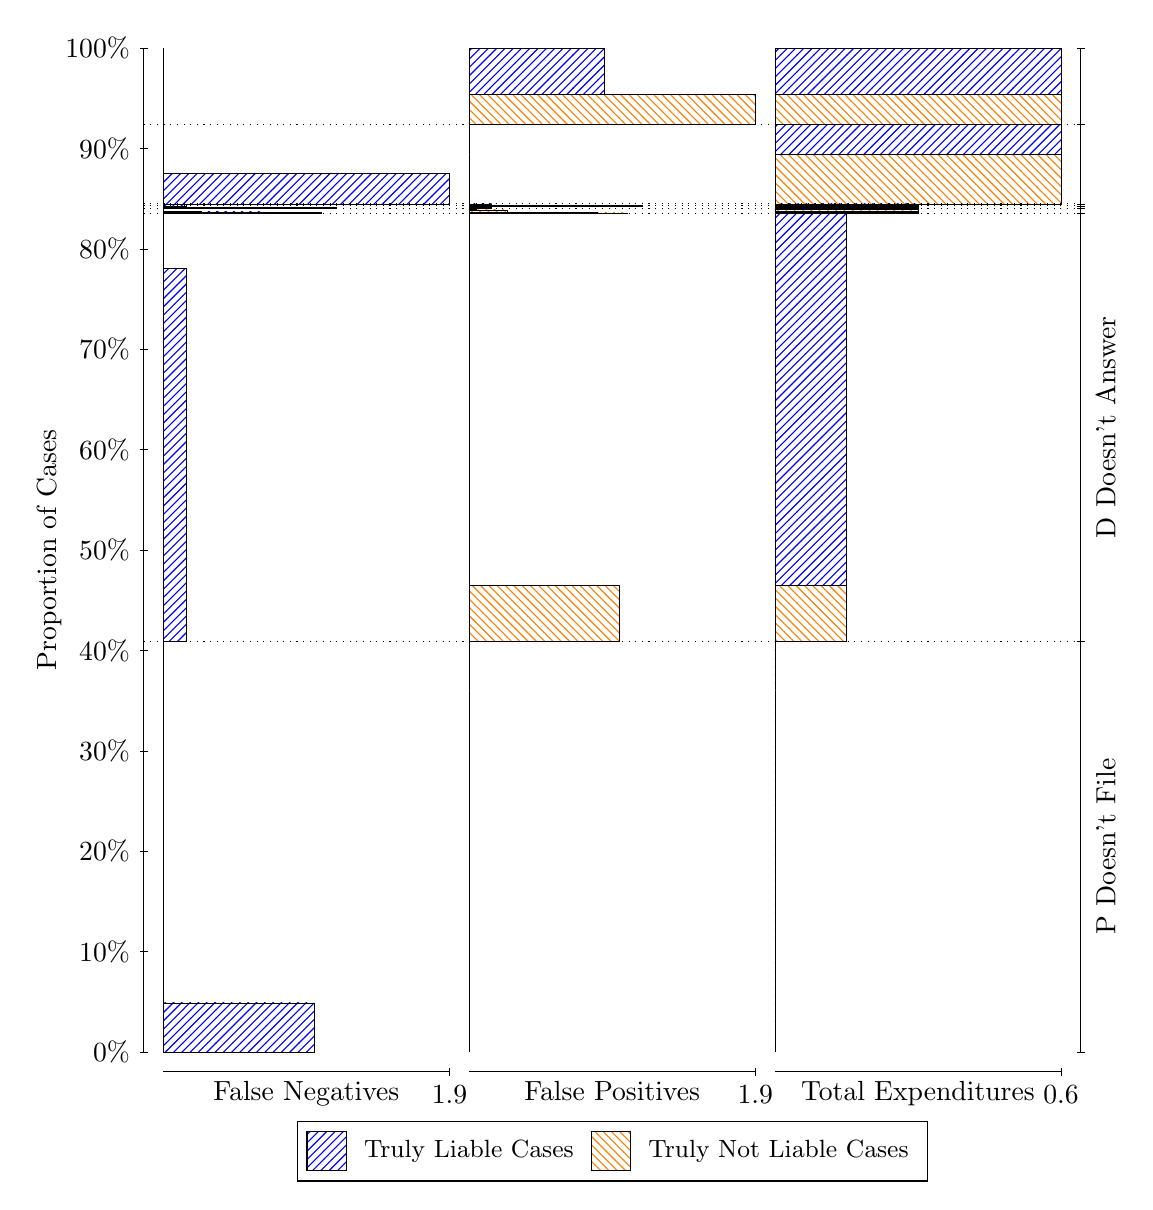
\begin{tikzpicture}
\draw[black, very thin] (1.5,1.75) -- (1.5,14.5);
\node[rotate=90, anchor=center] at (0.3, 8.125) {Proportion of Cases};
\draw[black, very thin] (1.45,1.75) -- (1.55,1.75);
\node[anchor=east] at (1.45, 1.75) {0\%};
\draw[black, very thin] (1.45,3.025) -- (1.55,3.025);
\node[anchor=east] at (1.45, 3.025) {10\%};
\draw[black, very thin] (1.45,4.3) -- (1.55,4.3);
\node[anchor=east] at (1.45, 4.3) {20\%};
\draw[black, very thin] (1.45,5.575) -- (1.55,5.575);
\node[anchor=east] at (1.45, 5.575) {30\%};
\draw[black, very thin] (1.45,6.85) -- (1.55,6.85);
\node[anchor=east] at (1.45, 6.85) {40\%};
\draw[black, very thin] (1.45,8.125) -- (1.55,8.125);
\node[anchor=east] at (1.45, 8.125) {50\%};
\draw[black, very thin] (1.45,9.4) -- (1.55,9.4);
\node[anchor=east] at (1.45, 9.4) {60\%};
\draw[black, very thin] (1.45,10.675) -- (1.55,10.675);
\node[anchor=east] at (1.45, 10.675) {70\%};
\draw[black, very thin] (1.45,11.95) -- (1.55,11.95);
\node[anchor=east] at (1.45, 11.95) {80\%};
\draw[black, very thin] (1.45,13.225) -- (1.55,13.225);
\node[anchor=east] at (1.45, 13.225) {90\%};
\draw[black, very thin] (1.45,14.5) -- (1.55,14.5);
\node[anchor=east] at (1.45, 14.5) {100\%};

\draw[black, very thin] (13.4,1.75) -- (13.4,14.5);
\draw[black, very thin] (13.35,1.75) -- (13.45,1.75);
\node[anchor=west] at (13.35, 1.75) {};
\draw[black, very thin] (13.35,6.9673) -- (13.45,6.9673);
\node[anchor=west] at (13.35, 6.9673) {};
\draw[black, very thin] (13.35,12.404) -- (13.45,12.404);
\node[anchor=west] at (13.35, 12.404) {};
\draw[black, very thin] (13.35,12.462) -- (13.45,12.462);
\node[anchor=west] at (13.35, 12.462) {};
\draw[black, very thin] (13.35,12.495) -- (13.45,12.495);
\node[anchor=west] at (13.35, 12.495) {};
\draw[black, very thin] (13.35,12.521) -- (13.45,12.521);
\node[anchor=west] at (13.35, 12.521) {};
\draw[black, very thin] (13.35,13.533) -- (13.45,13.533);
\node[anchor=west] at (13.35, 13.533) {};
\draw[black, very thin] (13.35,14.5) -- (13.45,14.5);
\node[anchor=west] at (13.35, 14.5) {};

\draw[black, very thin, pattern color=blue, pattern=north east lines] (1.75,1.75) rectangle (3.6623,2.3748);
\draw[black, very thin, pattern color=orange, pattern=north west lines] (1.75,2.3748) rectangle (1.75,6.9673);
\draw[black, very thin, pattern color=blue, pattern=north east lines] (1.75,6.9673) rectangle (2.0368,11.698);
\draw[black, very thin, pattern color=orange, pattern=north west lines] (1.75,11.698) rectangle (1.75,12.404);
\draw[black, very thin, pattern color=blue, pattern=north east lines] (1.75,12.404) rectangle (3.7579,12.412);
\draw[black, very thin, pattern color=blue, pattern=north east lines] (1.75,12.412) rectangle (3.5667,12.412);
\draw[black, very thin, pattern color=blue, pattern=north east lines] (1.75,12.412) rectangle (3.3754,12.412);
\draw[black, very thin, pattern color=blue, pattern=north east lines] (1.75,12.412) rectangle (3.1842,12.413);
\draw[black, very thin, pattern color=blue, pattern=north east lines] (1.75,12.413) rectangle (2.993,12.418);
\draw[black, very thin, pattern color=blue, pattern=north east lines] (1.75,12.418) rectangle (2.8018,12.418);
\draw[black, very thin, pattern color=blue, pattern=north east lines] (1.75,12.418) rectangle (2.6105,12.419);
\draw[black, very thin, pattern color=blue, pattern=north east lines] (1.75,12.419) rectangle (2.4193,12.42);
\draw[black, very thin, pattern color=blue, pattern=north east lines] (1.75,12.42) rectangle (2.2281,12.422);
\draw[black, very thin, pattern color=orange, pattern=north west lines] (1.75,12.422) rectangle (1.75,12.462);
\draw[black, very thin, pattern color=blue, pattern=north east lines] (1.75,12.462) rectangle (3.9491,12.475);
\draw[black, very thin, pattern color=orange, pattern=north west lines] (1.75,12.475) rectangle (1.75,12.495);
\draw[black, very thin, pattern color=blue, pattern=north east lines] (1.75,12.495) rectangle (2.0368,12.51);
\draw[black, very thin, pattern color=orange, pattern=north west lines] (1.75,12.51) rectangle (1.75,12.521);
\draw[black, very thin, pattern color=blue, pattern=north east lines] (1.75,12.521) rectangle (5.3833,12.908);
\draw[black, very thin, pattern color=orange, pattern=north west lines] (1.75,12.908) rectangle (1.75,13.533);
\draw[black, very thin, pattern color=orange, pattern=north west lines] (1.75,13.533) rectangle (1.75,13.914);
\draw[black, very thin, pattern color=blue, pattern=north east lines] (1.75,13.914) rectangle (1.75,14.5);
\draw[black, very thin, pattern color=orange, pattern=north west lines] (5.6333,1.75) rectangle (5.6333,6.3425);
\draw[black, very thin, pattern color=blue, pattern=north east lines] (5.6333,6.3425) rectangle (5.6333,6.9673);
\draw[black, very thin, pattern color=orange, pattern=north west lines] (5.6333,6.9673) rectangle (7.5456,7.6735);
\draw[black, very thin, pattern color=blue, pattern=north east lines] (5.6333,7.6735) rectangle (5.6333,12.404);
\draw[black, very thin, pattern color=orange, pattern=north west lines] (5.6333,12.404) rectangle (7.6412,12.406);
\draw[black, very thin, pattern color=orange, pattern=north west lines] (5.6333,12.406) rectangle (7.45,12.407);
\draw[black, very thin, pattern color=orange, pattern=north west lines] (5.6333,12.407) rectangle (7.2588,12.408);
\draw[black, very thin, pattern color=orange, pattern=north west lines] (5.6333,12.408) rectangle (7.0675,12.408);
\draw[black, very thin, pattern color=orange, pattern=north west lines] (5.6333,12.408) rectangle (6.8763,12.413);
\draw[black, very thin, pattern color=orange, pattern=north west lines] (5.6333,12.413) rectangle (6.6851,12.413);
\draw[black, very thin, pattern color=orange, pattern=north west lines] (5.6333,12.413) rectangle (6.6851,12.413);
\draw[black, very thin, pattern color=orange, pattern=north west lines] (5.6333,12.413) rectangle (6.4939,12.414);
\draw[black, very thin, pattern color=orange, pattern=north west lines] (5.6333,12.414) rectangle (6.3026,12.414);
\draw[black, very thin, pattern color=orange, pattern=north west lines] (5.6333,12.414) rectangle (6.1114,12.443);
\draw[black, very thin, pattern color=blue, pattern=north east lines] (5.6333,12.443) rectangle (5.7289,12.446);
\draw[black, very thin, pattern color=blue, pattern=north east lines] (5.6333,12.446) rectangle (5.6333,12.462);
\draw[black, very thin, pattern color=orange, pattern=north west lines] (5.6333,12.462) rectangle (5.9202,12.482);
\draw[black, very thin, pattern color=blue, pattern=north east lines] (5.6333,12.482) rectangle (5.6333,12.495);
\draw[black, very thin, pattern color=orange, pattern=north west lines] (5.6333,12.495) rectangle (7.8325,12.506);
\draw[black, very thin, pattern color=blue, pattern=north east lines] (5.6333,12.506) rectangle (5.9202,12.521);
\draw[black, very thin, pattern color=orange, pattern=north west lines] (5.6333,12.521) rectangle (5.6333,13.146);
\draw[black, very thin, pattern color=blue, pattern=north east lines] (5.6333,13.146) rectangle (5.6333,13.533);
\draw[black, very thin, pattern color=orange, pattern=north west lines] (5.6333,13.533) rectangle (9.2667,13.914);
\draw[black, very thin, pattern color=blue, pattern=north east lines] (5.6333,13.914) rectangle (7.3544,14.5);
\draw[black, very thin, pattern color=orange, pattern=north west lines] (9.5167,1.75) rectangle (9.5167,6.3425);
\draw[black, very thin, pattern color=blue, pattern=north east lines] (9.5167,6.3425) rectangle (9.5167,6.9673);
\draw[black, very thin, pattern color=orange, pattern=north west lines] (9.5167,6.9673) rectangle (10.425,7.6735);
\draw[black, very thin, pattern color=blue, pattern=north east lines] (9.5167,7.6735) rectangle (10.425,12.404);
\draw[black, very thin, pattern color=orange, pattern=north west lines] (9.5167,12.404) rectangle (11.333,12.413);
\draw[black, very thin, pattern color=blue, pattern=north east lines] (9.5167,12.413) rectangle (11.333,12.423);
\draw[black, very thin, pattern color=orange, pattern=north west lines] (9.5167,12.423) rectangle (11.333,12.453);
\draw[black, very thin, pattern color=blue, pattern=north east lines] (9.5167,12.453) rectangle (11.333,12.46);
\draw[black, very thin, pattern color=orange, pattern=north west lines] (9.5167,12.46) rectangle (11.333,12.461);
\draw[black, very thin, pattern color=blue, pattern=north east lines] (9.5167,12.461) rectangle (11.333,12.462);
\draw[black, very thin, pattern color=orange, pattern=north west lines] (9.5167,12.462) rectangle (11.333,12.482);
\draw[black, very thin, pattern color=blue, pattern=north east lines] (9.5167,12.482) rectangle (11.333,12.495);
\draw[black, very thin, pattern color=orange, pattern=north west lines] (9.5167,12.495) rectangle (11.333,12.506);
\draw[black, very thin, pattern color=blue, pattern=north east lines] (9.5167,12.506) rectangle (11.333,12.521);
\draw[black, very thin, pattern color=orange, pattern=north west lines] (9.5167,12.521) rectangle (13.15,13.146);
\draw[black, very thin, pattern color=blue, pattern=north east lines] (9.5167,13.146) rectangle (13.15,13.533);
\draw[black, very thin, pattern color=orange, pattern=north west lines] (9.5167,13.533) rectangle (13.15,13.914);
\draw[black, very thin, pattern color=blue, pattern=north east lines] (9.5167,13.914) rectangle (13.15,14.5);
\draw[black, dotted] (1.5,6.9673) -- (13.4,6.9673);
\draw[black, dotted] (1.5,12.404) -- (13.4,12.404);
\draw[black, dotted] (1.5,12.462) -- (13.4,12.462);
\draw[black, dotted] (1.5,12.495) -- (13.4,12.495);
\draw[black, dotted] (1.5,12.521) -- (13.4,12.521);
\draw[black, dotted] (1.5,13.533) -- (13.4,13.533);
\draw[black, very thin] (1.75,1.5) -- (5.3833,1.5);
\node[anchor=north] at (3.5667, 1.5) {False Negatives};
\draw[black, very thin] (5.3833,1.45) -- (5.3833,1.55);
\node[anchor=north] at (5.3833, 1.45) {1.9};

\draw[black, very thin] (5.6333,1.5) -- (9.2667,1.5);
\node[anchor=north] at (7.45, 1.5) {False Positives};
\draw[black, very thin] (9.2667,1.45) -- (9.2667,1.55);
\node[anchor=north] at (9.2667, 1.45) {1.9};

\draw[black, very thin] (9.5167,1.5) -- (13.15,1.5);
\node[anchor=north] at (11.333, 1.5) {Total Expenditures};
\draw[black, very thin] (13.15,1.45) -- (13.15,1.55);
\node[anchor=north] at (13.15, 1.45) {0.6};

\node[black, centered, rotate=90] at (13.72, 4.3586) {P Doesn't File};
\node[black, centered, rotate=90] at (13.72, 9.6858) {D Doesn't Answer};






\draw (7.449999999999999,1.5) node[draw=none] (baseCoordinate) {};
\begin{scope}[align=center]
        \matrix[scale=0.5, draw=black, below=0.5cm of baseCoordinate, nodes={draw}, column sep=0.1cm]{
            \node[rectangle, draw, minimum width=0.5cm, minimum height=0.5cm, pattern=north east lines, pattern color=blue] {}; &
            \node[draw=none, font=\small] (B) {Truly Liable Cases}; &
            \node[rectangle, draw, minimum width=0.5cm, minimum height=0.5cm, pattern=north west lines, pattern color=orange] {}; &
            \node[draw=none, font=\small] (B) {Truly Not Liable Cases}; \\
            };
\end{scope}

\end{tikzpicture}
\end{document}